% ========== MÅRHUND ==========
\begin{frame}{%
  \begin{minipage}[c]{0.30\textwidth}
    Mårhund
  \end{minipage}%
  \hfill
  \begin{minipage}[c]{0.45\textwidth}
    \footnotesize
    \textbf{Jagttid:} 1. sep -- 31. jan\\
    \textbf{Regulering:} Uden aftale (invasiv)
  \end{minipage}%
  \hfill
  \begin{minipage}[c]{0.15\textwidth}
    \noindent\raggedleft
    
\includegraphics[width=0.5cm, height=0.5cm, keepaspectratio]{Billeder/Ikoner/star.png}%
    \hspace{0.2em}%
    
\includegraphics[width=0.5cm, height=0.5cm, keepaspectratio]{Billeder/Ikoner/star.png}
  \end{minipage}%
}
  \vspace{0.25em}
  \begin{columns}[T]
    % --- Venstre kolonne: Tekst ---
    \column{0.45\textwidth}
    \setlength{\parskip}{0.4em}
    \tiny
    \RaggedRight
    \textbf{\textit{Nyctereutes procyonoides}} – invasivt hundedyr, der er ekstremt tilpasningsdygtigt. \par
    \textbf{Udseende:}\\
    \quad – Mørk med lange dækhår \\
    \quad – Bryst, ben og underside er sort \\
    \quad – Ansigtsmaske med brede sorte striber over øjnene \par
    \textbf{Levesteder:} Alle landskabstyper. \par
    \textbf{Føde:} Små pattedyr, fugle, fisk, bær, biller, ådsler, affald. \par
    \textbf{Udbredelse:} Primært Jylland.
    % --- Højre kolonne: Større billede ---
    \column{0.52\textwidth}
    \centering
    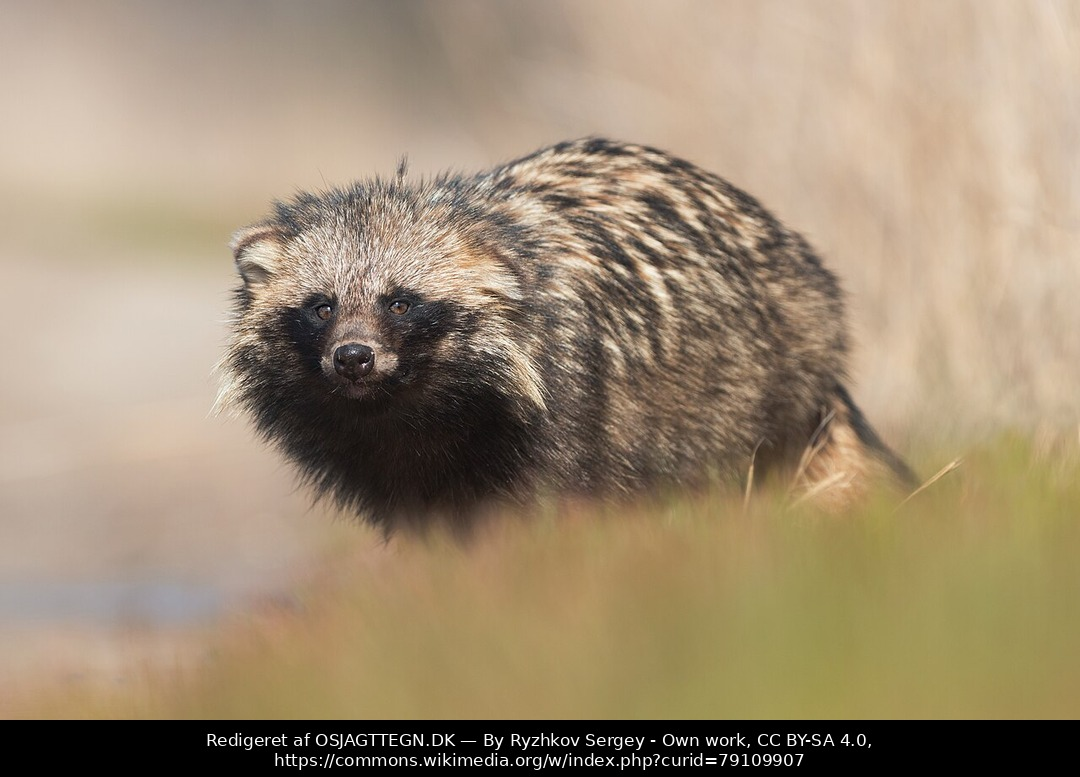
\includegraphics[width=\linewidth, height=7.2cm, keepaspectratio]{Billeder/Dyr/Pattedyr/rovdyr/mårhund/maarhund-01.jpg}
  \end{columns}
\end{frame}